\documentclass[12pt, a4paper]{article}

% --- Pakiety ---
\usepackage[utf8]{inputenc}
\usepackage[T1]{fontenc}
\usepackage[polish]{babel}
\usepackage{geometry}
\usepackage{amsmath}
\usepackage{amssymb}
\usepackage{graphicx}
\usepackage{booktabs}
\usepackage{siunitx}
\usepackage{caption}
\usepackage{subcaption}
\usepackage{float}
\usepackage{hyperref}
\usepackage{xcolor}
\usepackage{array}
\usepackage{multirow}
\usepackage{fancyhdr}

% --- Marginesy ---
\geometry{
    top=2.5cm,
    bottom=2.5cm,
    left=2.5cm,
    right=2.5cm
}

% --- Stopka ---
\pagestyle{fancy}
\fancyhf{}
\renewcommand{\headrulewidth}{0pt}
\renewcommand{\footrulewidth}{0.4pt}
\fancyfoot[R]{
\includegraphics[height=0.8cm]{lumon.pdf}}

% --- Konfiguracja siunitx ---
\sisetup{
    output-decimal-marker = {,},
    separate-uncertainty = true
}

% --- Dane raportu ---
\newcommand{\tytul}{Wyznaczanie prędkości dźwięku w cieczach metodą fali biegnącej}
\newcommand{\codeword}{Lucknow}
\newcommand{\nrCwiczenia}{F6}
\newcommand{\autor}{Karol Peszek}
\newcommand{\nrGrupy}{Grupa B}
\newcommand{\dataWykonania}{22 kwietnia 2026}

% --- Tytuł dokumentu ---
\title{
    \large I Pracownia Fizyczna \\[0.5em]
    \textbf{Ćwiczenie \nrCwiczenia} \\[0.3em]
    \LARGE \tytul\space''\codeword''
}
\author{
    \autor\\
     Grupa \nrGrupy}
\date{
    Data wykonania pomiarów: \dataWykonania\\
}

% =============================================
\begin{document}
% =============================================

\maketitle
\thispagestyle{empty}
\newpage

% -------------------------------------------
\section{Cel ćwiczenia}
% -------------------------------------------

Celem ćwiczenia jest wyznaczenie prędkości rozchodzenia się ultradźwięków w wodzie destylowanej oraz w wodnych roztworach chlorku sodu (NaCl) o znanych stężeniach masowych przy użyciu metody fali biegnącej. Na podstawie wyznaczonych prędkości zbadano zależność prędkości dźwięku od stężenia roztworu.

% -------------------------------------------
\section{Wstęp teoretyczny}
% -------------------------------------------

\subsection{Fala biegnąca w ośrodku sprężystym}

Zaburzenie mechaniczne elementu objętości ośrodka sprężystego powoduje jego drgania wokół położenia równowagi, które są przekazywane kolejnym warstwom ośrodka. Rozchodzące się w ten sposób zaburzenie nazywamy falą mechaniczną. Falę rozchodzącą się w kierunku osi $x$ opisuje równanie falowe:
\begin{equation}
    \frac{\partial^2 y}{\partial t^2} = u^2 \frac{\partial^2 y}{\partial x^2},
    \label{eq:wave}
\end{equation}
gdzie $u$ jest prędkością fazową fali. Rozwiązaniem równania (\ref{eq:wave}) jest fala harmoniczna o postaci:
\begin{equation}
    y = A\cos(\omega t - kx),
    \label{eq:harm}
\end{equation}
gdzie $A$ jest amplitudą, $\omega = 2\pi f$ częstotliwością kołową, a $k = 2\pi/\lambda$ liczbą falową. Prędkość fazową fali wyraża związek:
\begin{equation}
    u = \lambda f,
    \label{eq:speed}
\end{equation}
gdzie $\lambda$ jest długością fali, a $f$ jej częstotliwością. Fale, dla których prędkość fazowa nie zależy od częstotliwości, nazywamy falami niedyspersyjnymi.

\subsection{Fale podłużne w cieczach}

Ze względu na kierunek drgań cząstek ośrodka względem kierunku rozchodzenia się fali rozróżnia się fale podłużne (drgania równoległe do kierunku propagacji) i poprzeczne (drgania prostopadłe). Ciecze wykazują jedynie sprężystość objętościową, dlatego mogą przewodzić wyłącznie fale podłużne. Prędkość rozchodzenia się fali podłużnej w cieczy zależy od jej modułu ściśliwości $B$ oraz gęstości $\rho$:
\begin{equation}
    u = \sqrt{\frac{B}{\rho}}.
    \label{eq:elastic}
\end{equation}
W praktyce prędkość ta zależy od ciśnienia, temperatury i składu cieczy. Dla czystych cieczy zależność od temperatury jest w dobrym przybliżeniu liniowa. W przypadku roztworów wodnych NaCl prędkość dźwięku rośnie ze stężeniem, a zależność ta jest liniowa dla stężeń masowych do około $25\%$.

\subsection{Ultradźwięki i przetworniki piezoelektryczne}

Falami dźwiękowymi nazywamy podłużne fale mechaniczne o częstotliwościach z zakresu słyszalnego przez człowieka, tj.\ od około $20\,\mathrm{Hz}$ do $20\,\mathrm{kHz}$. Fale o częstotliwościach powyżej tej granicy to ultradźwięki. W niniejszym ćwiczeniu stosuje się generator pracujący przy częstotliwości $f = 2\,\mathrm{MHz}$.

Do wytwarzania i detekcji ultradźwięków używa się przetworników piezoelektrycznych. Zjawisko piezoelektryczne polega na tym, że odkształcenie mechaniczne kryształu (np.\ kwarcu) powoduje pojawienie się na jego powierzchniach ładunku elektrycznego, a przyłożone pole elektryczne wywołuje odkształcenie mechaniczne. Pozwala to na wzajemną konwersję sygnałów elektrycznych i akustycznych.

\subsection{Metoda fali biegnącej --- krzywe Lissajous}

W metodzie fali biegnącej głowica nadawcza zanurzana jest w badanej cieczy i wytwarza falę ultradźwiękową, która rozchodzi się w kierunku głowicy odbiorczej. Sygnał z generatora podawany jest na wejście $X$ oscyloskopu, a sygnał z głowicy odbiorczej --- na wejście $Y$. Na ekranie oscyloskopu obserwuje się krzywą Lissajous powstającą ze złożenia dwóch sygnałów harmonicznych o tej samej częstotliwości:
\begin{equation}
    y_G = A\cos\!\left[2\pi\!\left(\frac{t}{T} - \frac{x_0}{\lambda}\right) + \delta\right], \qquad
    y_M = A\cos\!\left[2\pi\!\left(\frac{t}{T} - \frac{x_0 + r}{\lambda}\right) + \delta\right],
\end{equation}
gdzie $r$ jest odległością między głowicami, a $\delta$ przesunięciem fazowym. Różnica faz między sygnałami wynosi $\Delta = 2\pi r/\lambda$. Gdy $\Delta = n\pi$ (dla $n = 0, 1, 2, \ldots$), elipsa degeneruje się do odcinka prostej. Kolejne takie degeneracje odpowiadają przesunięciu głowicy odbiorczej o połowę długości fali $\lambda/2$. Mierząc położenia śruby mikrometrycznej przy kolejnych degeneracjach, wyznacza się długość fali $\lambda$, a następnie prędkość dźwięku ze wzoru (\ref{eq:speed}).



% -------------------------------------------
\section{Opis układu pomiarowego}
% -------------------------------------------
\begin{figure}[H]
    \centering
    
\includegraphics[width=\textwidth]{schema.jpg}
    \caption{Fotografia układu pomiarowego.}\label{fig:schema}
\end{figure}

\subsection{Dostępne przyrządy i materiały}
Do przeprowadzenia pomiarów wykorzystano następujące przyrządy i materiały:
\begin{itemize}
    \item generator GWINSTEK MFG-2110, umożliwiający wytwarzanie sygnałów o częstotliwości $2\,\mathrm{MHz}$.
    \item oscyloskop InfiniiVision KEYSIGHT EDUX1002A, służący do obserwacji krzywych Lissajous.
    \item uchwyt z zamocowanymi głowicami nadawczą i odbiorczą, oraz ceramicznym naczyniem i śrubą mikrometryczną do precyzyjnego ustawiania odległości między głowicami.
    \item woda destylowana oraz wodne roztwory chlorku sodu (NaCl) o stężeniach masowych $10\%$, $20\%$.
    \item izolowane przewody koncentryczne do połączenia głowic z oscyloskopem i generatorem.
\end{itemize}

\subsection{Przygotowanie układu pomiarowego}
\begin{enumerate}
    \item Przygotować roztwory NaCl o stężeniach masowych $10\%$ i $20\%$ poprzez dokładne odważenie odpowiednich ilości NaCl i wody destylowanej, a następnie dokładne wymieszanie.
    \item Zamocować głowicę nadawczą i odbiorczą w uchwycie, tak aby były ustawione naprzeciwko siebie i mogły być precyzyjnie przesuwane za pomocą śruby mikrometrycznej.
    \item Napełnić ceramiczne naczynie wodą destylowaną i umieścić w nim głowice, tak aby były całkowicie zanurzone.
    \item Podłączyć głowicę nadawczą do generatora, a głowicę odbiorczą do oscyloskopu, używając izolowanych przewodów koncentrycznych.
    \item Ustawić generator na częstotliwość $2\,\mathrm{MHz}$ i odpowiednią amplitudę sygnału, tak aby na oscyloskopie pojawiła się wyraźna krzywa Lissajous.
\end{enumerate}

% -------------------------------------------
\section{Procedura pomiarowa}
% -------------------------------------------
W celu wyznaczenia prędkości dźwięku w badanych cieczach, przeprowadzono następujące kroki pomiarowe dla każdej z cieczy (woda destylowana, roztwór NaCl $10\%$, roztwór NaCl $20\%$):
\begin{enumerate}
    \item Dokładnie opłukać i osuszyć naczynie i głowice przed każdym pomiarem, aby uniknąć zanieczyszczeń i zapewnić powtarzalność wyników.
    \item Umieścić głowice w naczyniu z badaną cieczą, tak głowice były bardzo blisko siebie.
    \item Napełnić naczynie badaną cieczą, tak aby głowice były całkowicie zanurzone.
    \item Ustawić położenie głowicy odbiorczej tak, aby na oscyloskopie pojawiła się krzywa Lissajous w zdegenerowanej formie (odcinek prostej), co odpowiada sytuacji, gdy różnica faz między sygnałami wynosi $\Delta = n\pi$.
    \item Zarejestrować położenie śruby mikrometrycznej dla kolejnych degeneracji krzywej Lissajous, aż do uzyskania 20 pomiarów.
    \item Powtórzyć powyższe kroki dla pozostałych cieczy, pamiętając o dokładnym oczyszczeniu naczynia i głowic przed każdym pomiarem.
\end{enumerate}


% -------------------------------------------
\section{Wyniki pomiarów}
% -------------------------------------------

Częstotliwość generatora ultradźwięków wynosiła $f = \SI{2.000000e6}{\hertz}$ i przyjęta jest jako dokładna ($u_f = 0$). Dla każdego ośrodka zarejestrowano $N = 20$ kolejnych położeń $r_i$ śruby mikrometrycznej odpowiadających degeneracjom krzywej Lissajous do odcinka, co odpowiada kolejnym wielokrotnościom $\lambda/2$. Niepewność każdego pomiaru położenia przyjęto jako $u_r = \SI{0.01}{\milli\metre}$ (działka elementarna śruby).

\begin{table}[H]
\centering
\caption{Zmierzone położenia śruby mikrometrycznej $r_i$ dla kolejnych degeneracji krzywej Lissajous. Wszystkie wartości w \si{\milli\metre}, $u_r = \SI{0.01}{\milli\metre}$.}\label{tab:raw}
\begin{tabular}{c
    S[table-format=1.2]
    S[table-format=1.2]
    S[table-format=1.2]}
\toprule
$i$ & {Woda destylowana} & {NaCl $10\%$} & {NaCl $20\%$} \\
    & {$r_i$ [\si{\milli\metre}]} & {$r_i$ [\si{\milli\metre}]} & {$r_i$ [\si{\milli\metre}]} \\
\midrule
 1 &  0.31 &  0.17 &  0.74 \\
 2 &  0.65 &  0.55 &  1.16 \\
 3 &  1.03 &  0.95 &  1.59 \\
 4 &  1.41 &  1.35 &  2.02 \\
 5 &  1.77 &  1.75 &  2.45 \\
 6 &  2.15 &  2.16 &  2.88 \\
 7 &  2.52 &  2.56 &  3.30 \\
 8 &  2.89 &  2.96 &  3.73 \\
 9 &  3.27 &  3.36 &  4.16 \\
10 &  3.64 &  3.77 &  4.59 \\
11 &  4.01 &  4.17 &  5.02 \\
12 &  4.39 &  4.57 &  5.44 \\
13 &  4.76 &  4.97 &  5.88 \\
14 &  5.13 &  5.37 &  6.30 \\
15 &  5.50 &  5.77 &  6.72 \\
16 &  5.87 &  6.17 &  7.16 \\
17 &  6.24 &  6.57 &  7.57 \\
18 &  6.62 &  6.98 &  7.99 \\
19 &  6.99 &  7.38 &  8.45 \\
20 &  7.37 &  7.78 &  8.88 \\
\bottomrule
\end{tabular}
\end{table}

Zależność mierzonego położenia od numeru pomiaru powinna być liniowa ze współczynnikiem kierunkowym równym $\lambda/2$. Wykres surowych danych przedstawiony jest na rysunku~\ref{fig:raw}.

\begin{figure}[H]
    \centering
    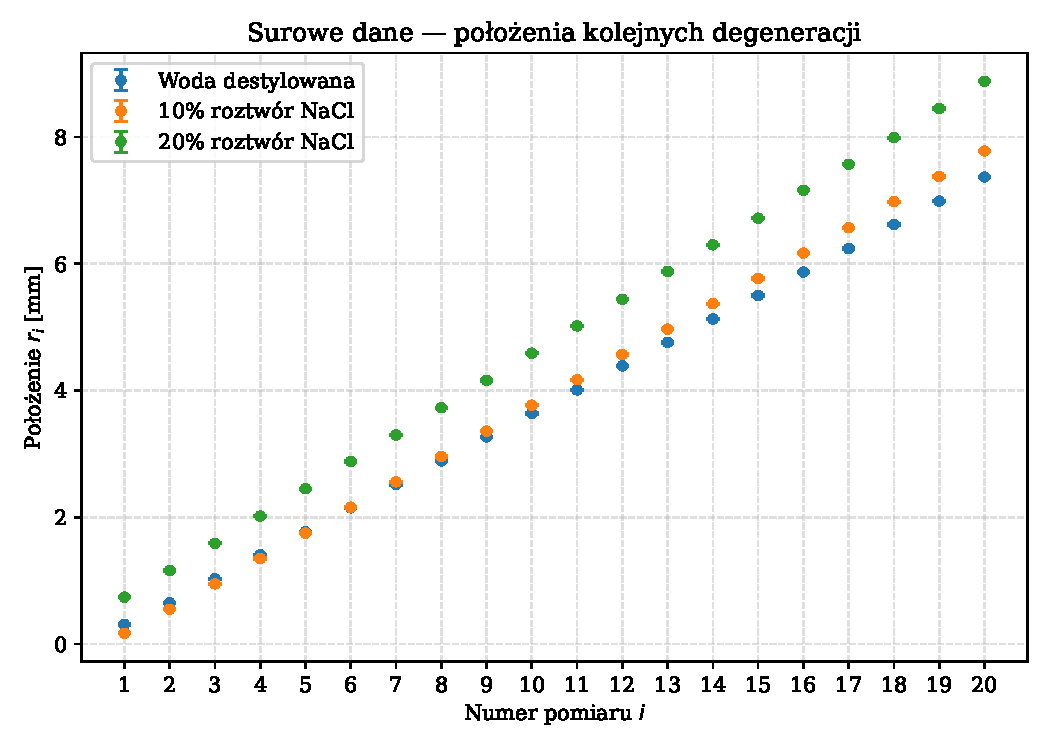
\includegraphics[width=0.82\textwidth]{raw_data.pdf}
    \caption{Zmierzone położenia śruby mikrometrycznej $r_i$ w funkcji numeru pomiaru $i$ dla trzech badanych ośrodków. Słupki błędów odpowiadają niepewności $u_r = \SI{0.01}{\milli\metre}$.}\label{fig:raw}
\end{figure}



% -------------------------------------------
\section{Opracowanie wyników}
% -------------------------------------------

\subsection{Wyznaczanie długości fali}

Kolejne zarejestrowane położenia $r_i$ odpowiadają kolejnym wielokrotnościom $\lambda/2$. Wszystkie $N = 20$ pomiarów wykorzystano optymalnie, dopasowując prostą regresji liniowej metodą najmniejszych kwadratów:
\begin{equation}
    r_i = A\cdot i + B, \qquad i = 1, 2, \ldots, 20,
    \label{eq:regr}
\end{equation}
gdzie $A = \lambda/2$ jest współczynnikiem kierunkowym. Długość fali i jej niepewność wyznaczane są jako:
\begin{equation}
    \lambda = 2A, \qquad u_\lambda = 2\,u_A,
    \label{eq:lam_regr}
\end{equation}
gdzie $u_A$ jest standardowym błędem współczynnika kierunkowego wynikającym z~regresji.

Wyznaczone wartości zestawiono w tabeli~\ref{tab:lambda}. Dopasowanie regresji wraz z residuami przedstawiono na rysunku~\ref{fig:fit}.

\begin{figure}[H]
    \centering
    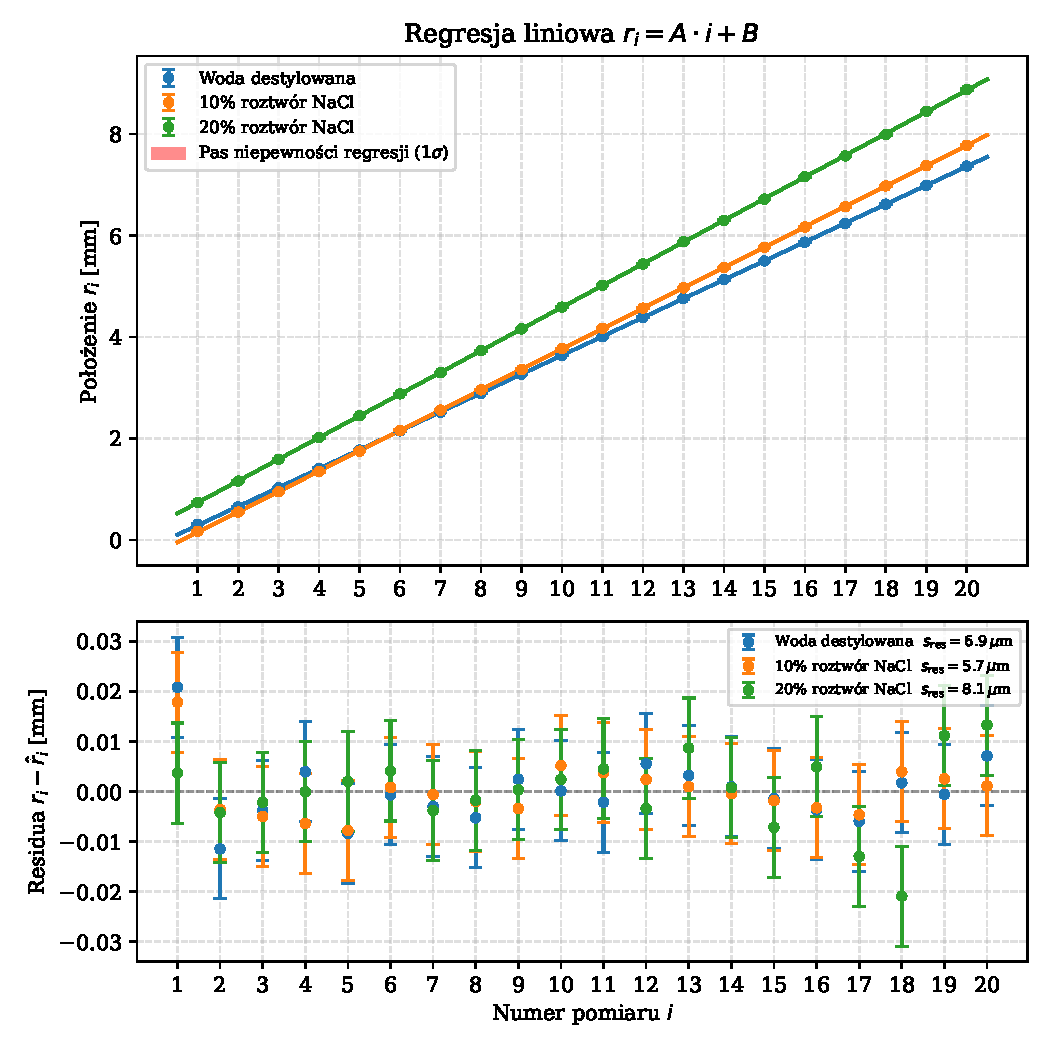
\includegraphics[width=0.88\textwidth]{regression_fit.pdf}
    \caption{Górny panel: dopasowanie regresji liniowej $r_i = A\cdot i + B$ do danych pomiarowych; czerwone pasy: przedział ufności prostej regresyjnej ($1\sigma$). Dolny panel: residua $r_i - \hat{r}_i$; w legendzie podano odchylenie standardowe reszt $s_{\rm res}$ dla każdego ośrodka.}\label{fig:fit}
\end{figure}

\begin{table}[H]
\centering
\caption{Długość fali $\lambda = 2A$ i jej niepewność $u_\lambda = 2u_A$ wyznaczone z regresji liniowej~\eqref{eq:regr}--\eqref{eq:lam_regr}.}\label{tab:lambda}
\begin{tabular}{l
    S[table-format=1.4]
    S[table-format=1.4]}
\toprule
Ośrodek & {$\lambda$ [\si{\milli\metre}]} & {$u_\lambda$ [\si{\milli\metre}]} \\
\midrule
Woda destylowana & 0.7446 & 0.0005 \\
NaCl $10\%$      & 0.8028 & 0.0004 \\
NaCl $20\%$      & 0.8558 & 0.0006 \\
\bottomrule
\end{tabular}
\end{table}

\subsection{Wyznaczanie prędkości dźwięku}

Prędkość dźwięku w danym ośrodku wyznaczana jest ze wzoru~(\ref{eq:speed}):
\begin{equation}
    v = f \cdot \lambda.
    \label{eq:v}
\end{equation}
Ponieważ częstotliwość $f$ przyjmowana jest jako dokładna ($u_f = 0$), niepewność prędkości wynika wyłącznie z niepewności długości fali:
\begin{equation}
    u_v = f \cdot u_\lambda.
    \label{eq:u_v}
\end{equation}

Wyznaczone prędkości zestawiono w tabeli~\ref{tab:velocity}. Na rysunku~\ref{fig:vel} przedstawiono je w formie wykresu słupkowego.

\begin{table}[H]
\centering
\caption{Prędkość dźwięku $v$ i jej niepewność $u_v$ dla każdego ośrodka.}\label{tab:velocity}
\begin{tabular}{l
    S[table-format=4.1]
    S[table-format=1.1]}
\toprule
Ośrodek & {$v$ [\si{\metre\per\second}]} & {$u_v$ [\si{\metre\per\second}]} \\
\midrule
Woda destylowana & 1489.2 & 1.1 \\
NaCl $10\%$      & 1605.6 & 0.9 \\
NaCl $20\%$      & 1711.7 & 1.3 \\
\bottomrule
\end{tabular}
\end{table}

\begin{figure}[H]
    \centering
    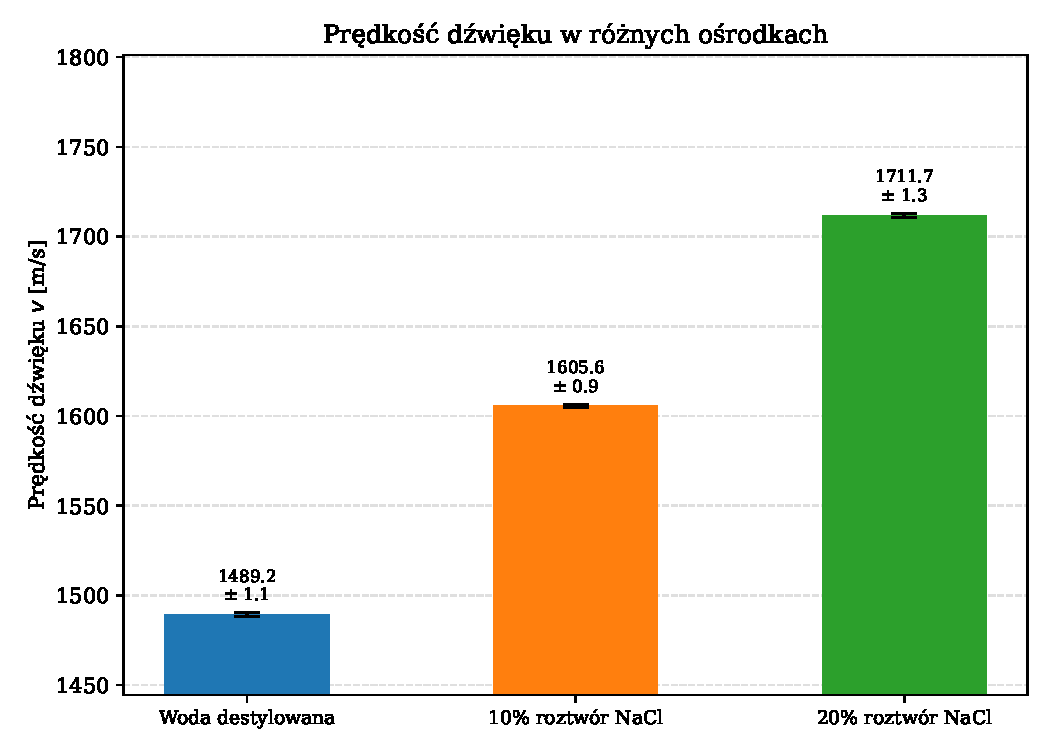
\includegraphics[width=0.78\textwidth]{velocities.pdf}
    \caption{Prędkość dźwięku $v$ w badanych ośrodkach. Słupki błędów odpowiadają niepewności $u_v$ wyznaczonej ze wzoru~(\ref{eq:u_v}).}\label{fig:vel}
\end{figure}



% -------------------------------------------
\section{Wnioski}
% -------------------------------------------

Wyznaczone prędkości dźwięku wykazują wyraźną, monotoniczną zależność od stężenia masowego roztworu NaCl.
Wzrost stężenia z $0\%$ (woda destylowana) do $10\%$ powoduje wzrost prędkości o~ok.\ $116\,\mathrm{m/s}$, a~dalszy wzrost do $20\%$ --- o~kolejne ok.\ $106\,\mathrm{m/s}$, co potwierdza niemal liniowy charakter tej zależności w~badanym zakresie stężeń~\cite{chen1978}.

Wyznaczona prędkość dźwięku w~wodzie destylowanej
\[
  v_{\text{H}_2\text{O}} = (1489{,}2 \pm 1{,}1)\,\mathrm{m/s}
\]
jest zgodna z~wartością tabelaryczną wynikającą z~równania Chena i~Millero dla czystej wody~\cite{chen1978}: $U_w^0 \approx 1488{,}3\,\mathrm{m/s}$ w~temperaturze $\approx 22\,^{\circ}\mathrm{C}$ --- różnica mieści się w~granicach $1\sigma$.

Dla roztworu NaCl 10\% (molalność $m \approx 1{,}90\,\mathrm{mol/kg}$) wartość literaturowa wyznaczona ze wzoru empirycznego Chena, Chena i~Millero~\cite{chen1978} wynosi $U_{\text{lit}} \approx 1601\,\mathrm{m/s}$, zaś zmierzona prędkość
\[
  v_{10\%} = (1605{,}6 \pm 0{,}9)\,\mathrm{m/s}
\]
odbiega od niej o~ok.\ $4{,}6\,\mathrm{m/s}$, czyli około $5\sigma$ niepewności statystycznej..
Rozbieżność ta może wynikać z~odmiennej temperatury pomiaru (dokładna wartość nie była monitorowana) oraz niedokładności przygotowania roztworów.

Dla roztworu NaCl 20\% (molalność $m \approx 4{,}28\,\mathrm{mol/kg}$) zastosowanie wzoru empirycznego~\cite{chen1978} wykracza poza deklarowany zakres walidacji ($m \leq 1\,\mathrm{mol/kg}$), dlatego bezpośrednie porównanie nie jest w~pełni miarodajne; ekstrapolacja daje $\approx 1726\,\mathrm{m/s}$, co odbiega od zmierzonego
\[
  v_{20\%} = (1711{,}7 \pm 1{,}3)\,\mathrm{m/s}
\]
o~ok.\ $14\,\mathrm{m/s}$, zgodnie z~oczekiwanym wzrostem błędu ekstrapolacji poza zakres danych referencyjnych.

Dominującym źródłem niepewności statystycznej był rozrzut odczytów śruby mikrometrycznej ($s_{res} \approx 7$--$8\,\mu\mathrm{m}$). Całkowita niepewność pomiaru jest jednak prawdopodobnie zdominowana przez czynniki systematyczne (niemonitorowana temperatura, precyzja przygotowania roztworów), co wynika z obserwowanej rozbieżności z wartościami literaturowymi. Temperatura, niemonitorowana bezpośrednio, mogła wprowadzić błąd rzędu kilku m/s.


% -------------------------------------------
\begin{thebibliography}{9}
% -------------------------------------------

\bibitem{chen1978}
C.\nobreakdash-T.\ Chen, L.\nobreakdash-S.\ Chen, F.\ J.\ Millero,
\textit{Speed of sound in NaCl, MgCl$_2$, Na$_2$SO$_4$, and MgSO$_4$ aqueous
solutions as functions of concentration, temperature, and pressure},
J.\ Acoust.\ Soc.\ Am.\ \textbf{63} (6), 1795--1800 (1978).
Dostępne: \url{https://www.researchgate.net/publication/243501733}

\bibitem{skrypt}
\textit{Skrypt do ćwiczeń laboratoryjnych z fizyki, I Pracownia Fizyczna}, ćwiczenie F6.
\end{thebibliography}

\end{document}
% =============================================
